\section{Giảm chiều đặc trưng bằng PCA}
\label{sec:4_4}
PCA được đặt sau khi ghép hai nhánh. Bước này tự center đầu vào đã xử lý và không whitening; không có bước scale bổ sung cho từng cột one-hot. Các hướng chiếu và số thành phần được học từ train, dùng bộ giải SVD đầy đủ.

Cấu hình cơ sở có 105 đặc trưng. PCA 90\% giữ 22 thành phần và 90,70\% phương sai train; PCA 95\% giữ 31 thành phần và 95,12\% phương sai. Đây là kết quả kiểm tra đặc trưng, chưa phải so sánh chất lượng phân loại.

\begin{figure}[htbp]
\centering
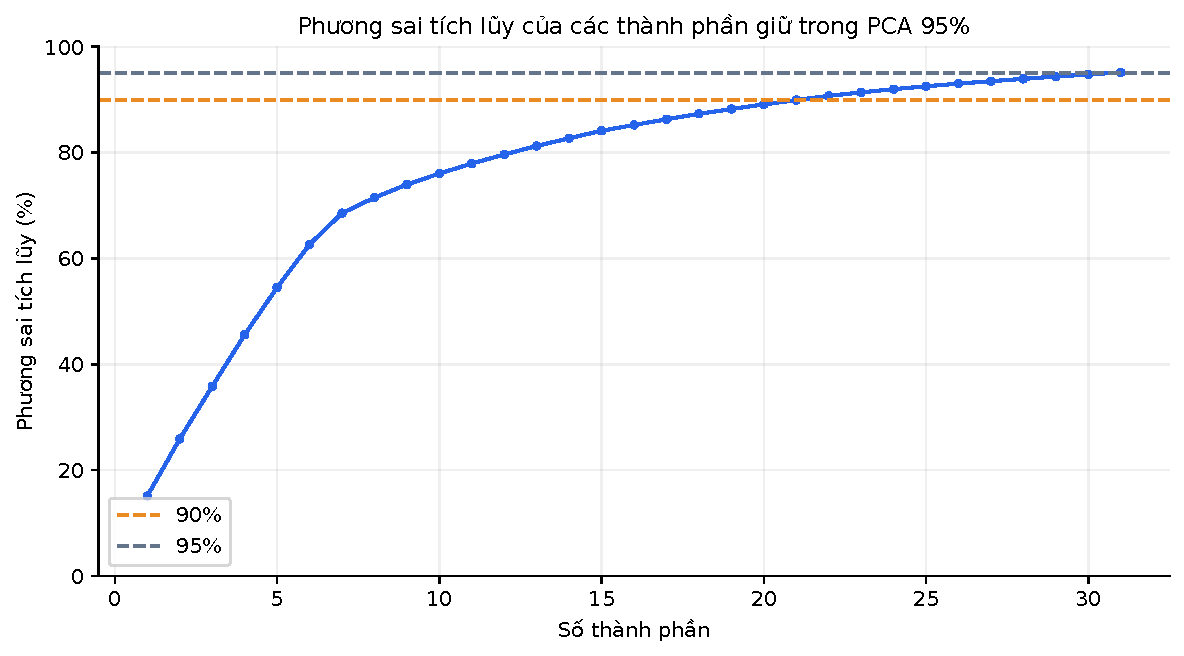
\includegraphics[width=.9\textwidth]{Images/chapter_4/4_4/pca_cumulative_variance.pdf}
\caption{Phương sai tích lũy của những thành phần được giữ trong cấu hình PCA 95\%}
\label{fig:pca-retained-variance}
\end{figure}
